\documentclass[tikz, border=10pt]{standalone}
\usepackage{tikz}
\usetikzlibrary{arrows.meta, positioning, fit, backgrounds, calc}

\definecolor{colInput}{RGB}{173,214,241}
\definecolor{colNorm} {RGB}{200,200,200}
\definecolor{colConv} {RGB}{130,179,220}
\definecolor{colDense}{RGB}{253,192,134}
\definecolor{colZoom} {RGB}{220,235,220}

\tikzset{
  base/.style  = {draw, rounded corners=3pt, font=\small, align=center,
                  inner sep=4pt, minimum height=7mm, minimum width=40mm},
  zinput/.style= {base, fill=colInput},
  zop/.style   = {base, fill=colNorm},
  zmlp/.style  = {base, fill=colDense, minimum width=36mm},
  zres/.style  = {base, fill=red!40, minimum width=36mm},
  arr/.style   = {-{Stealth[length=5pt]}, thick},
}

\begin{document}
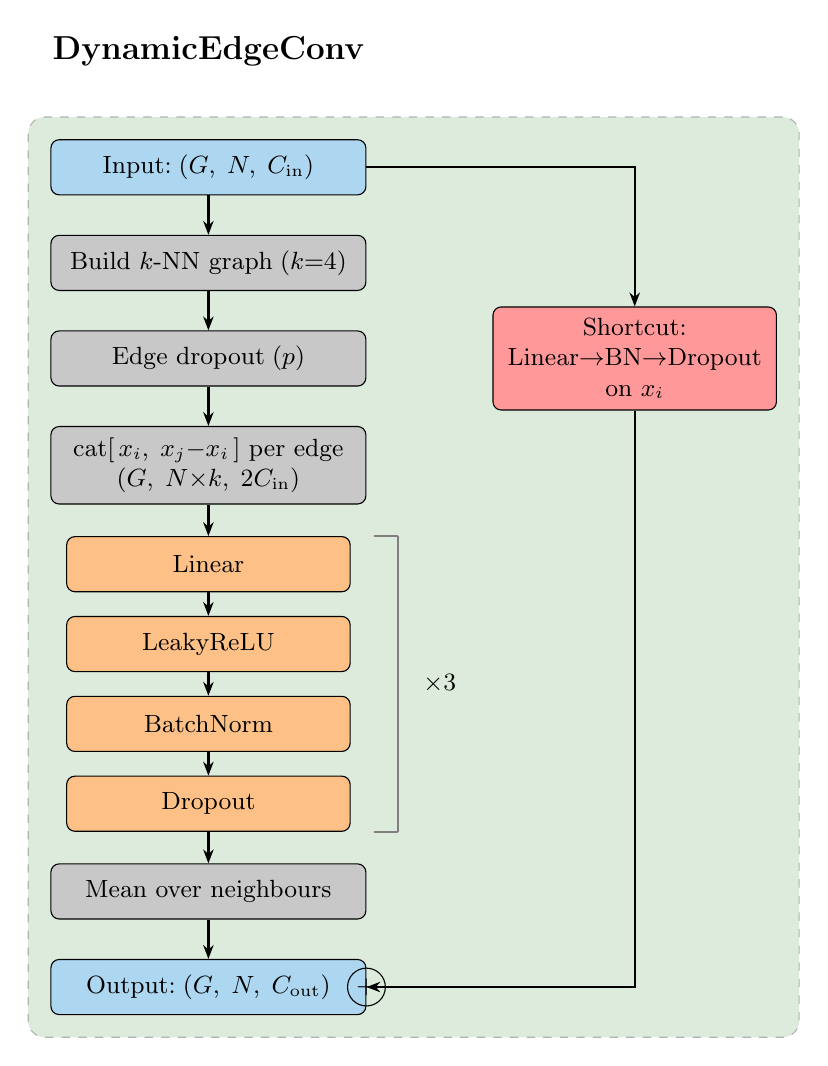
\begin{tikzpicture}[node distance=5mm]

%% ── title ───────────────────────────────────────────────────────────────────
\node[font=\large\bfseries] (title) {DynamicEdgeConv};

%% ── nodes ───────────────────────────────────────────────────────────────────
\node[zinput, below=8mm of title]  (zin)   {Input:\;$(G,\;N,\;C_{\rm in})$};
\node[zop,    below=5mm of zin]    (zknn)  {Build $k$-NN graph\;($k{=}4$)};
\node[zop,    below=5mm of zknn]   (zdrop) {Edge dropout\;($p$)};
\node[zop,    below=5mm of zdrop]  (zcat)  {cat$[\,x_i,\;x_j{-}x_i\,]$ per edge\\$(G,\;N{\times}k,\;2C_{\rm in})$};
\node[zmlp,   below=4mm of zcat]   (zm1)   {Linear};
\node[zmlp,   below=3mm of zm1]    (zm2)   {LeakyReLU};
\node[zmlp,   below=3mm of zm2]    (zm3)   {BatchNorm};
\node[zmlp,   below=3mm of zm3]    (zm4)   {Dropout};
\node[zop,    below=4mm of zm4]    (zagg)  {Mean over neighbours};
\node[zinput, below=5mm of zagg]   (zout)  {Output:\;$(G,\;N,\;C_{\rm out})$};

%% ── shortcut (right side) ───────────────────────────────────────────────────
\node[zres, right=16mm of zdrop] (zsc)
  {Shortcut:\\Linear$\to$BN$\to$Dropout\\on $x_i$};

%% ── main arrows ─────────────────────────────────────────────────────────────
\draw[arr] (zin)   -- (zknn);
\draw[arr] (zknn)  -- (zdrop);
\draw[arr] (zdrop) -- (zcat);
\draw[arr] (zcat)  -- (zm1);
\draw[arr] (zm1)   -- (zm2);
\draw[arr] (zm2)   -- (zm3);
\draw[arr] (zm3)   -- (zm4);
\draw[arr] (zm4)   -- (zagg);
\draw[arr] (zagg)  -- (zout);

%% ── shortcut arrows ─────────────────────────────────────────────────────────
\draw[arr] (zin.east)  -| (zsc.north);
\draw[arr] (zsc.south) |- (zout.east);

%% ── ] x3 bracket on right of MLP block ──────────────────────────────────────
\draw[thick, gray]
  ([xshift=6mm]zm1.north east) -- ([xshift=6mm]zm4.south east)
  ([xshift=6mm]zm1.north east) -- ([xshift=3mm]zm1.north east)
  ([xshift=6mm]zm4.south east) -- ([xshift=3mm]zm4.south east);
\node[font=\small, anchor=west] at ([xshift=8mm]$(zm1.east)!0.5!(zm4.east)$)
  {$\times 3$};

%% ── add symbol at output junction ───────────────────────────────────────────
\node[draw, circle, inner sep=1.5pt, font=\small] at (zout.east) {$+$};

%% ── background panel ────────────────────────────────────────────────────────
\begin{pgfonlayer}{background}
  \node[draw=gray!60, dashed, fill=colZoom, rounded corners=6pt,
        fit=(zin)(zout)(zsc), inner sep=8pt] {};
\end{pgfonlayer}

\end{tikzpicture}
\end{document}
